% !TEX root = ../paper.tex

\section{Method}

\subsection{Problem Formulation}

We study RGB-thermal registration as a scene-level alignment task. For each scene, the input is a
set of paired RGB and thermal UAV frames
$S = \{(I_i^R, I_i^T)\}_{i=1}^N$, where viewpoint variation, cross-resolution sensing, thermal
appearance changes, and day/night conditions make individual frame estimates uneven in quality. The
goal is to recover a thermal-to-RGB homography that remains reliable at the scene level, with the
canonical output retained when the evidence satisfies the reliability criterion.

This formulation turns registration from a single best-pair problem into a multi-frame reliability
optimization problem. In our setting, many scenes already contain usable pairwise correspondences,
but the central challenge is to convert uneven frame-level estimates into a transform that is
geometrically stable, internally consistent, and acceptable under a reliability-aware criterion.

\begin{figure}[t]
\centering
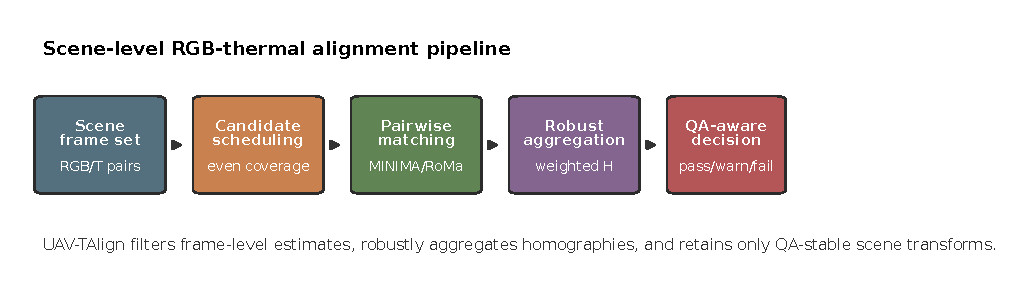
\includegraphics[width=\textwidth]{figures/fig_method_pipeline.pdf}
\caption{Overview of UAV-TAlign. The framework builds on strong pairwise matching, but
makes the final decision at the scene level through reliability-guided evidence selection, robust
homography consensus, and QA-aware verification.}
\label{fig:method_pipeline}
\end{figure}

\subsection{Pairwise Evidence Backbone}

UAV-TAlign uses a strong off-the-shelf multimodal matcher as its pairwise evidence generator. Our
PRCV implementation uses the MINIMA family with the RoMa branch as the default backend, while the
rest of the pipeline remains agnostic to the exact pairwise matcher
\cite{edstedt2024roma,ren2025minima}.

\subsection{Reliability-Guided Evidence Selection}

At the scene level, UAV-TAlign prioritizes the most informative frame evidence before expanding the
support set. It uses a progressive evidence schedule that expands with scene size and can cover all
frames when needed. This reliability-guided policy allows the framework to stop when a compact
subset already yields a stable consensus, while still escalating to broader evidence when the scene
benefits from more support.

Within each stage, representative frames are selected with deterministic evenly distributed
sampling by default. A random-selection variant is used only for sensitivity analysis. The default
policy is therefore framed as a reproducible operating choice that reduces seed-dependent drift and
preserves uniform scene coverage.

\subsection{Quality-Weighted Frame Geometry}

For each selected frame pair, the matcher produces cross-modal correspondences that are filtered
into a frame-level homography estimate. UAV-TAlign evaluates each frame using
standard geometric statistics, including the number of matches, the number of inliers, inlier
ratio, reprojection error, and spatial coverage. A frame enters the global candidate pool only when
it passes a geometry-quality gate on these statistics. The overall geometric treatment remains rooted
in standard homography estimation and robust fitting practice
\cite{hartley2004multiple,fischler1981ransac,barath2019magsac,barath2020magsacpp}.

Beyond a binary accept/reject decision, the pipeline assigns each accepted frame a quality score so
that better-supported homographies receive more influence during scene aggregation. The score is a
weighted combination of inlier ratio, spatial coverage, reprojection quality, matcher confidence,
and inlier count. This keeps the scene-level estimate from being dominated by low-support frames
that only marginally satisfy the frame-level gate.

\subsection{Robust Scene Consensus}

Once enough frame-level homographies have been accepted, UAV-TAlign forms a scene-level consensus.
Homographies are mapped into parameter space, centered with a median reference, and filtered by a
median-absolute-deviation rule to suppress unstable estimates before weighted averaging. The
retained homographies are then combined using the frame quality scores defined above.

The pipeline records stability diagnostics around the aggregate transform, including homography
dispersion relative to the aggregate and the ratio of robustly rejected frame-level estimates.
These diagnostics connect consensus formation with the final QA-aware decision.

\subsection{QA-Aware Scene Verification}

The final decision integrates match availability with scene-level reliability evidence. UAV-TAlign
evaluates the optimized scene-level transform against a label-free QA summary computed on
representative frames. The current summary uses cross-modal proxy signals such as edge-overlap
improvement, gradient-NCC improvement, the ratio of improved frames, and the count of severe
relative outliers. It also retains scene-level match and stability statistics such as accepted-frame
ratio, mean inlier ratio, mean reprojection error, spatial coverage, dispersion relative to the
aggregate transform, and the robust reject ratio.

The canonical decision uses a baseline-aware verification rule. A scene is retained when
accepted-frame statistics remain strong, the aggregated homography is stable, severe
baseline-relative outliers remain controlled, and the transform improves gradient-based alignment
beyond configured floors. This final verification step gives UAV-TAlign its scene-level character:
the framework optimizes for reliable alignment products rather than merely maximizing the number of
matched frames.
